\documentclass[a4paper,11pt]{refart}
\usepackage{listingsutf8}
\usepackage[brazilian]{babel}
\usepackage[utf8]{inputenc}
\usepackage[T1]{fontenc} % LY1 also works
\usepackage{tikz}
\usetikzlibrary{shapes,arrows}
%% Font settings suggested by fbb documentatio
\usepackage{float} 
\usepackage{listings}
\usepackage{microtype}
\usepackage{graphicx}
\usepackage{enumitem}
\hyphenation{Trans-fe-rên-cias} %Hifenação de palavras
\setlist{leftmargin=*}
\lstset{basicstyle=\ttfamily,frame=single,xleftmargin=1em,xrightmargin=1em}
\usepackage[os=win]{menukeys}
\renewmenumacro{\keys}[+]{shadowedroundedkeys}
\usepackage{framed}
\usepackage{etoolbox}
\AtBeginEnvironment{leftbar}{\sffamily\small}
\usepackage[T1]{fontenc}
\usepackage{lmodern}
\usepackage{hyperref}
\usepackage{multirow}                                               
\usepackage{multicol}                                               
\usepackage{longtable}
\usepackage{amsmath,amssymb,mathtools,amsfonts,textcomp}
\usepackage{dcolumn}
\usepackage{booktabs}
\usepackage{makecell}
\usepackage{tablefootnote}
\everymath{\displaystyle}
\hypersetup{colorlinks=true,linkcolor=black,citecolor=blue,urlcolor=blue}

\renewcommand\theadalign{bc}
\renewcommand\theadfont{\bfseries}
\renewcommand\theadgape{\Gape[4pt]}
\renewcommand\cellgape{\Gape[4pt]}

\renewcommand\abstractname{}
\def\CS#1{\texttt{\textbackslash#1}}

\usepackage[most]{tcolorbox}
\newtcblisting{commandshell}{colback=black,colupper=green,colframe=black!75!black,
	listing only,listing options={style=tcblatex,language=sh},
	every listing line={\textcolor{red}{\small\ttfamily\bfseries pc@user:\$ }}}

\usepackage[most]{tcolorbox}
\newtcblisting{shell}{colback=black,colupper=green,colframe=black!75!black,
	listing only,listing options={style=tcblatex,language=sh},
	every listing line={\textcolor{red}{\small\ttfamily\bfseries}}}


\title{PRIMoRDiA: Guia do Usuário 1.25v  }
\author{Igor Barden Grillo \\(\url{barden.igor@gmail.com} )\\\url{github.com/igorChem}}
	
\begin{document}
\maketitle

\begin{abstract}
\hspace*{-1.4\leftmarginwidth}
\begin{minipage}{\fullwidth}
\begin{figure}[H]
	\begin{center}
		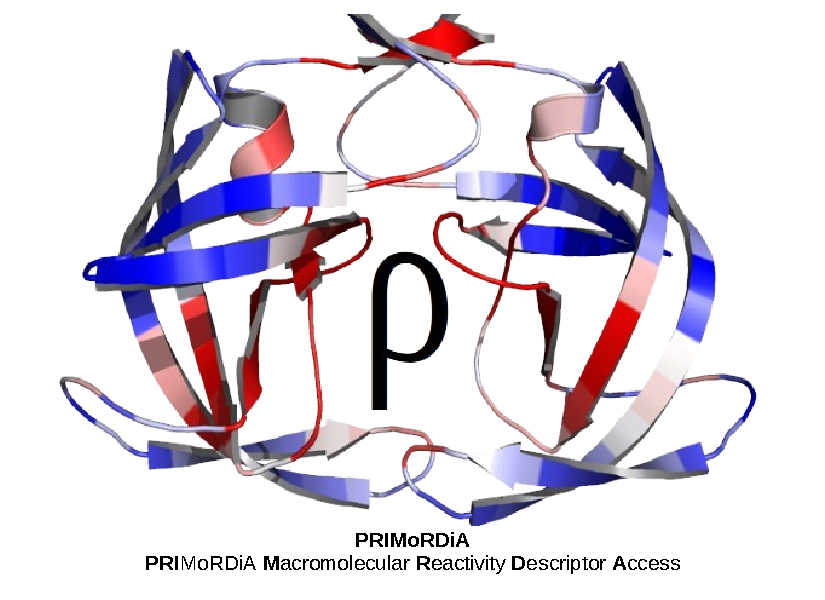
\includegraphics[width=7in]{logo_primordia}
	\end{center}
\end{figure}

\end{minipage}

\end{abstract}
\newpage
\tableofcontents
\newpage

\section{Introdução}

PRIMoRDiA ( \textbf{PRI}MoRDiA \textbf{M}acromolecular \textbf{R}eactivity \textbf{D}escriptors \textbf{A}ccess ) é um software escrito em \emph{C++}, desenvolvido para o pós-processamento eficiente de resultados de pacotes de química computacional, produzindo uma grande variedade de descritores quânticos, que são propriedades eletrônicas e de reatividade dos sistemas químicos. 

O PRIMoRDiA traz implementado os principais descritores de reatividade da Teoria do DFT conceitual, incluindo as definições matemáticas para as teorias de elétrons de fronteira de Fukui e de Ácidos e Bases Duros e Moles de Pearson. O PRIMoRDiA foi desenvolvido com foco no cálculo para grandes moléculas que são relevantes para processos biológicos, e por isso há descritores modificados especificamente para atender as particularidades desses sistemas. 

Esse guia traz informações gerais sobre a teoria por de trás dos descritores, e detalha o uso e a interpretação dos resultados gerados pelo programa. Para mais informações nós encorajamos o contato através dos e-mails fornecidos no repositório e nesse documento. PRIMoRDiA foi desenvolvido na Universidade Federal da Paraíba, no Laboratório de Química Quântica e Computacional.

Este Guia do Usuário esta em constante modificação. Novas versões dele serão disponibilizadas conforme identificado as necessidades dos usuários e novas funcionalidades sendo implementadas no programa.

\section{Download e Instalação}

PRIMoRDiA é um software de código livre sob a licença pública Mozilla 2.0. No repositório do Git Hub nós fornecemos versões estáveis do programa, com todos os arquivos fonte, dados para teste e binários já compilados. Nós indicamos fortemente a compilação do programa usando o \emph{CMake}. 

O programa foi desenvolvido para sistemas operacionais Linux, visando usuários acostumados a trabalhar na área de modelagem molecular. No entanto, para fins didáticos e de divulgação, é fornecido código e binário para o sistema Windows em outro repositório: \url{https://github.com/igorChem/PRIMoRDiA_WIN64}. Lembrando que não há um suporte constante para essa versão.

Para baixar os dados do repositório é possível usar o seguinte comando do git:

\hspace*{-\leftmarginwidth}
\begin{minipage}{\fullwidth}
	\begin{commandshell}git clone https://github.com/igorChem/PRIMoRDiA1.0v.git\end{commandshell}
\end{minipage}

Através desse comando, a pasta do repositório vai ser baixada no diretório de onde o seu terminal está aberto, podendo ser atualizado facilmente com o comando: 

\hspace*{-\leftmarginwidth}
\begin{minipage}{\fullwidth}
	\begin{commandshell}git pull\end{commandshell}
\end{minipage}

Também, no próprio site é possível baixar um '.zip' contendo todos os dados do repositório. 
No entanto, é fortemente recomentado que o usuário baixe uma das versões estáveis, de preferência a última. Essas versões estáveis tem a garantia de estarem com todas as suas funcionalidades devidamente testadas. 

\emph{\textbf{PRIMoRDiA é um programa que está em constante desenvolvimento e clonar o repositório em qualquer outro ponto que não seja as marcadas como estáveis pode gerar erros na utilização. }}

Link para última versão: \url{https://github.com/igorChem/PRIMoRDiA1.0v/releases/tag/v1.25}

\subsection{ Compilação com CMake (mais indicado) }

A compilação com o CMake é muito simples de se realizar, com poucos comandos é gerado um binário do PRIMoRDiA otimizado para a sua máquina. A desvantagem da compilação em relação a utilização dos binários prontos é a necessidade de instalação de algumas bibliotecas exigidas pelo PRIMoRDiA. Às vezes, o usuário também não tem os compiladores e o próprio CMake para o processo de compilação. 

Em distribuições Linux mais populares baseadas em Debian, como por exemplo Ubuntu e Mint, isso pode ser facilmente resolvido instalando as bibliotecas a partir do repositório.

Por padrão, o PRIMoRDiA utiliza o g++-8 e a biblioteca Eigen 3. Para assegurar que sua máquina tenha o necessário para compilar o PRIMoRDiA, execute os comandos abaixo

\hspace*{-\leftmarginwidth}
\begin{minipage}{\fullwidth}
\begin{commandshell}
sudo apt install g++-8 
sudo apt install cmake
sudo apt install libeigen3-dev
\end{commandshell}
\end{minipage}
 
Depois de descomprimir a pasta baixada com a versão estável entre no diretório e faça a compilação usando os seguintes comandos: 

\hspace*{-\leftmarginwidth}
\begin{minipage}{\fullwidth}
\begin{commandshell}cd /caminho/da/pasta/PRIMoRDiA1.0v
cmake .
make
\end{commandshell}
\end{minipage}

O processo de compilação deve ocorrer sem problemas e gerar um arquivo binário chamado "PRIMoRDIA\_1.25v\_LINUX64 ", caso a versão 1.25 seja a escolhida ( mais recomendado ).
Com a linha de código mostrada abaixo é possível criar um atalho no arquivo ".bashrc" para executar o programa de qualquer diretório do seu sistema

\hspace*{-\leftmarginwidth}
\begin{minipage}{\fullwidth}
\begin{commandshell}
alias primordia='caminho/PRIMoRDiA1.0v/PRIMoRDiA\_1.25v\_LINUX64'
\end{commandshell}
\end{minipage}


\subsection{Binários Compilados} 

No caso da impossibilidade de compilação, binários para a última versão estável é fornecido no repositório. O mesmo processo de colocar no caminho pode ser realizado. Problemas de falta de alguma biblioteca compartilhada podem acontecer, assim como a performance máxima não ser alcançada. Entretanto, qualquer problema com a execução dos binários é encorajado que os mesmos sejam reportados. 

\newpage
\section{Versões do Programa}

Até o momento da divulgação desse Guia de Usuário, o programa possui três versões estáveis. 
As mudanças que aparacem de forma mais sensível ao usuário estão no formato do input e na quantidade de dados extraído pelo software. O ideal é sempre dar preferência para a última versão estável. 

\begin{enumerate}
	\item \textbf{1.0v}:\\
	Nove descritores globais e quatorze locais implementados. Descritores para macromoléculas, com descritores assinalados individualmente para residuos de proteínas e DNA (formato do PDB).  
	\item \textbf{1.2v}:
	\\ Novo modelo de input, com mais controle; Scripts de R para análise estatística de trajetória de reação e dinâmica molecular, enfoque em análise nos átomos da coordenada de reação e residuos requeridos no input. Ajustes gerais no código. 
	\item \textbf{1.25v}: Mais três métodos de dureza local implementados, e os mesmos descritores locais implementados para representação volumétrica e condensada. Ajustes na automatização de visualização dos resultados no Pymol. Correções e padronização de nomenclatura. 
\end{enumerate}

\newpage
\section{Descritores de Reatividade: Teoria}

Os descritores de reatividade (DR) são quantidades teóricas que são convenientes para resumir propriedades de reatividade de sistemas moleculares, como um todo ou de diferentes regiões e/ou átomos. Os DRs de mais sucesso na literatura são os baseados na Conceptual Density Functional Theory (CDFT), que consegue englobar diferentes teorias de reatividade química através de definições matemáticas extraídas do DFT, relacionando essas quantidade com conceitos químicos já bem estabelecidos\cite{geerlings2003conceptual}. 

Esses descritores são obtidos da densidade eletrônica calculada a partir de sistemas moleculares, sendo propriedades que só podem ser obtidas a partir de cálculos quânticos. Outras propriedades eletrônicas, como a própria densidade eletrônica, energia total e cargas parciais, são exemplos de quantidades calculáveis a partir da densidade eletrônica e podem servir de descritores. O conjunto de todas essas propriedades calculadas pelo PRIMoRDiA são chamadas pelo nosso grupo de Descritores Quânticos Moleculares (DQM) ou só Descritores Quânticos.

Os DRs definidos dentro da CDFT provem da equação diferencial total do DFT (\autoref{eq.1}) e suas derivadas\cite{parr1978elect}, que relaciona a energia eletrônica ($E$) com a densidade eletrônica ($\rho(r)$) do estado de referência e o potencial externo ($\nu(r)$). Os DR da CDFT podem ser classificado como sendo globais, um número que representa um propriedade eletrônica para todo o sistema, ou locais, uma função da posição do sistema. 

\begin{equation}
dE = \mu dN + \int \rho(r) d \nu (r) dr
\label{eq.1}
\end{equation}

Como os principais descritores são derivadas, o cálculo se dá através de dois métodos de aproximação, que no caso são a Aproximação de Orbitais Congelados (AOC) e de Diferenças Finitas (DF). Os descritores locais podem ser separados ainda pelo método de representação/visualização, Condensado para átomos ou em uma representação volumétrica de uma grade tridimensional, com cada voxel representada por um valor. Esse esquema de classificação dos descritores pode ser visualizado na \autoref{fig:M1}.

\tikzstyle{block} = [rectangle, draw, fill=cyan!20, 
text width=5em, text centered, rounded corners, minimum height=4em]
\tikzstyle{decision} = [diamond, draw, fill=yellow!20, 
text width=4.5em, text badly centered, node distance=3cm, inner sep=0pt]
\tikzstyle{line} = [draw, -latex']

\begin{figure}[H]
	\centering
\begin{tikzpicture}[node distance = 2.5cm, auto]
\node [block] (init) {CDFT Descritores};
\node [decision, below of=init] (typerd) {DR Escopo};
\node [block, right of=typerd] (local) {Local};
\node [block, left of=typerd] (global) {Global};
\node [decision, right of=local] (rep) {Vis.};
\node [block, above of=rep] (cond) {Condensado};
\node [block, below of=rep] (vol) {3D Grid};
\node [decision, below of=typerd] (method) {Método};
\node [block, right of=method] (foa) {AOC};
\node [block, left of=method] (fd) {DF};
\path [line] (init) -- (typerd); 
\path [line] (typerd) -- (local); 
\path [line] (typerd) -- (global); 
\path [line] (global) -- (method);
\path [line] (local) -- (method);
\path [line] (local) -- (rep);
\path [line] (method) -- (foa);
\path [line] (method) -- (fd);
\path [line] (rep) -- (cond);
\path [line] (rep) -- (vol);
\end{tikzpicture}
\caption{Classificação dos descritores de Reatividade do CDFT.} \label{fig:M1}
\end{figure}


\subsection{Descritores Globais}

O potencial químico eletrônico (PQE) é um exemplo de descritor de reatividade global, que no DFT é o multiplicador de Lagrange (representado pela letra $\mu$) que minimiza a energia eletrônica em relação a densidade, dado o potencial externo constante. Na tabela \autoref{tab1} é apresentada a definição matemática para os descritores de reatividade global e as formas de cálculo nos dois métodos de aproximação.  

\hspace*{-\leftmarginwidth}
\begin{minipage}{\fullwidth}
	\begin{table}[H]
		\centering	
		\caption{Descritores de Reatividade implementados no PRIMoRDiA}
		\begin{tabular}{c|c|c|c|c}
			\toprule
			DR global & Definição em CDFT  & AOC & DF & Ref. \\
			\midrule
			IP & -  & $- E_{HOMO}$ & $E_{N-1}-E_{N}$  &  \\  \hline	
			EA & -  & $- E_{LUMO}$ & $E_{N}-E_{N+1}$ & \\ \hline	
			$\mu$  & $\left(\frac{\partial E}{\partial N} \right)_\nu$  & $\frac{E_{HOMO} + E_{LUMO}}{2}$ &$\frac{E_{N-1}-E_{N+1}}{2}$ & \cite{ribeiro2017atlas}\\ \hline			
			$\eta$  & $\left(\frac{\partial ^2  E}{\partial N ^2} \right)_\nu$ &$E_{LUMO} - E_{HOMO}$ &$E_{N-1}+E_{N+1}-2E_{N}$ & \cite{parr1983absolute}\\ \hline
			Softness($S$)  & $1/\eta$  & - & -  & \cite{parr1983absolute} \\ \hline
			$\omega$  & $\frac{\mu^2S}{2}$  &-  &-  & \cite{cedillo2012local} \\ \hline
			$nMax$  & $-\frac{\omega}{\eta} $ & - & - & \cite{cedillo2012local}  \\ 
			\bottomrule
		\end{tabular} 
		\label{tab1}	
	\end{table}	
\end{minipage}


O PQE estabelece a propensão dos sistema de doar elétrons, e quando os valores entre diferentes sistemas moleculares se igualam a transferência de elétrons cessa, caracterizando o estado de equilíbrio\cite{parr1983absolute}. Por causa disso é que $\mu$ é batizado em analogia ao potencial químico molar da termodinâmica clássica. 

O princípio de Ácidos e Bases Duros e Moles  (\textit{HSAB: Hard and Soft Acid and Base}) de Pearson\cite{pearson1987recent} é uma das teorias de reatividade química que ganhou fundamentação teórica e matemática dentro do CDFT. Pearson criou conceitos batizados de dureza e moleza química para explicar a afinidade entre ácidos e bases pelo modelo de Lewis, baseado na observação de características atômicas e moleculares e as séries de reatividade\cite{Pearson1963}. Desse estudo foi definido que ácidos Duros são pequenos receptores de elétrons e pouco polarizáveis, que por sua vez tendem a interagir quimicamente com bases duras, que são doadores de elétrons com as mesmas características de volume e polarizabilidade. Essa interação entre espécies consideradas quimicamente "duras" por Pearson ocorrem por interações controladas por carga, formando ligações de caráter iônico. 

Já os ácidos e bases moles são espécies polarizáveis e volumosas, onde a interação é governada pela deslocalização dos orbitais moleculares de fronteira, havendo uma doação de elétrons do orbital ocupado de mais alta energia (HOMO) da base para o orbital virtual de mais baixa energia do ácido (LUMO). Nesse processo de interação de espécies moles há uma transferência de carga líquida da base para o ácido e também tendo maior chance de formação de ligações com caráter covalente. Logo, é possível estabelecer regras complementares para entender as principais forças que levam uma reação química a acontecer usando esse principio de Pearson.

No entanto, até a consolidação do CDFT, o HSAB era uma teoria sem respaldo matemático e uma forma sistemática de determinar escalar de dureza e moleza. No CDFT, a dureza é primeiramente encarada como uma propriedade do sistema que representa a sua resistência em doar elétrons, sendo também a característica de sistemas pouco polarizáveis e de pequeno volume, ou seja, onde os elétrons ficam mais aglutinados aos núcleos.

A definição matemática do descritor global associada a dureza química no CDFT é a derivada do PQE em respeito ao número de elétrons, o mesmo que a derivada segunda da energia em respeito do número de elétrons, e comumente representado com a letra grega $\eta$. Rapidamente, a moleza química global é definida como o recíproco da dureza, normalmente representado pela letra $S$.

Outros descritores globais que podem são obtidos no CDFT são basicamente sobre esses processos de transferência de carga, que geralmente são utilizados para racionalizar reações químicas. Como por exemplo: O máximo número de elétrons que podem ser recebidos por um sistema por um doador ideal $nMax$; a estabilização de energia quando o sistema recebe esse número de elétrons, que pode ser chamado de eletrofilicidade e representado na literatura do CDFT com a letra grega $\omega$\cite{Pearson1990}.  

\subsection{Métodos de Cálculo}

Como já citado acima, a maioria dos descritores de reatividade são derivadas da energia e/ou da densidade eletrônica em respeito ao número de elétrons. O número de elétrons é sempre inteiro, e portanto não exite uma função continua dessa quantidade, sendo necessário que essas derivadas sejam aproximados através de métodos matemáticos. 

O método mais comum para a determinação numérica de derivadas, seja qual for, é o métodos de diferenças finitas (DF). Para as quantidade do CDFT, os cálculos tem que ser realizados utilizando dados da estrutura eletrônica de três estados de carga do sistema. Para os descritores globais, as informações necessárias são as energias eletrônicas desses três estados de carga, o estado de referência, o carregado positivamente (pelo menos um elétrons a menos) e o carregado negativamente (pelo menos um elétron a mais).

Para os descritores locais essa lógica se aplica da mesma forma para a densidade eletrônica, ou carga parcial no caso da representação condensada por átomos. Todos os cálculos de estrutura eletrônica devem ser realizados para as mesmas coordenadas atômicas do estado de referência, isto é, para a mesma posição dos núcleos, respeitando a condição de potencial externo constante requerido por essas derivadas.  

O outro método de cálculo é chamado de Aproximação de Orbitais Congelados (\textit{Frozen Orbital Approximation} em inglês)\cite{yang1984electron}, que utiliza as informações dos orbitais moleculares de fronteira, HOMO e LUMO, e desconsidera a variação de energia/distribuição espacial dos orbitais internos, o que justifica o nome do método. 

Para os descritores globais em particular, os cálculos são realizados com a energia dos orbitais moleculares HOMO e LUMO, e também é conhecido como Teorema de Koopmans\cite{manne1970koopmans}, que estabelece que a energia do HOMO é a aproximação do Potencial de Ionização (PI) e a energia do LUMO como sendo a aproximação dda Afinidade Eletrônica (AE). A grande diferença é dessa aproximação para a de diferenças finitas é que só requer uma avaliação de estrutura eletrônica (comumente chamado de \textit{Single Point} em inglês). E em relação aos descritores locais, a obtenção das densidades de probabilidade desses orbitais requer um esforço computacional irrisório frete ao necessário para a densidade eletrônica total. 

Logo, AOC tem um custo computacional significativamente menor que o DF, sendo o último se tornando proibitivo para grandes moléculas. Quanto a acurácia, a aproximação de DF por definição é teoricamente maior, já que considera a perturbação de toda a densidade eletrônica quando o sistema participa de processos de transferência de carga. No entanto, a AOC é estimada por orbitais moleculares que geralmente tem grande importância na explicação da reatividade química das moléculas, pois da a distribuição de probabilidade de localização dos elétrons que são mais suscetíveis aos processos químicos.   


\subsection{Descritores Locais}

A definição matemática de um descritor local é uma função do espaço tridimensional $r$, ou seja, dado um ponto no espaço o descritor assume certo valor. A densidade eletrônica $\rho$ é uma dessas quantidades locais por definição, onde o valor da densidade é definida pelo produto dos orbitais moleculares ocupados $\phi_{occ}(r)$ (\autoref{eq.2}), que por sua vez são combinações lineares de orbitais atômicos $\phi $, onde os coeficientes $c_i$ são determinados por métodos de química computacional. 

\begin{equation}
\rho(r) = \sum_{i}^{occ} |\psi(r)^2_i|
\label{eq.2} 
\end{equation}

\begin{equation}
\psi(r)_i = \sum_{i} c_i \phi(r)
\label{eq.3} 
\end{equation}

\subsubsection{Métodos de Representação}

A forma prática de representar esses descritores locais é definir uma grade tridimensional, onde cada ponto $r$ relaciona coordenadas tridimensionais do sistema químico com um valor. Esses pontos são conhecidos como \textit{voxel}, o análogo tridimensional do pixel, e geralmente são reunidos em um arquivo formatado chamado de \textit{Gaussian Cube}, ou simplesmente cube, com a extensão ".cube". Esse arquivo tem um padrão que é reconhecido pela grande maioria dos softwares de visualização molecular, podendo a partir deles criar representações gráficas de iso-superfícies, renderizar mais de uma dessas iso-superfícies atribuindo diferentes cores e opacidades, o que resulta em uma representação volumétrica. 

Dentro da linguagem dos descritores quânticos adotada pelo PRIMoRDiA, essa representação é conhecida como volumétrica. O PRIMoRDiA calcula 21 propriedades eletrônica/descritores de reatividade que podem ser escritas no disco como arquivos Cube formatados. Para isso, é necessário que o usuário defina a resolução da grade tridimensional diferente de zero e forneça os dados de estrutura eletrônica necessários para o cálculo desses descritores quânticos. Mais detalhes sobre os parâmetros, input e os descritores em si são dados nas próximas sessões desse guia. 

Como já dito antes, cada voxel representa um valor do descritor local para um dado ponto $r$. Para facilitar a interpretação química e manipulação numérica dessas propriedades é possível integrar elas em uma base comum $\Omega$. Como por exemplo, uma fração da densidade eletrônica pode ser atribuída a um átomo do sistema molecular através de uma análise populacional, como a de Muliken ou Lowdin por exemplo. Esses métodos numéricos somam os coeficientes dos orbitais moleculares, ou elementos da matriz densidade, que são atribuídos aos orbitais atômicos, particionando esses valores para cada átomo. Esse processo é conhecido como condensação, gerando uma representação condensada para átomos, e geralmente abreviada para somente "condensada". 

No caso genérico mostrado na \autoref{eq.4}, o descritor $f(r)$ pode ter parte sua atribuída ao átomo $k$ através da integração dos valores de $f(r)$ nas funções de base referente a esse átomo. O PRIMoRDiA calcula os descritores e escreve um arquivo com a lista de valores dos descritores locais ordenadas pelo índice dos átomos no arquivo fornecido para o software. 

\begin{equation}
f_k^{a} = \int_{\Omega k} f(r)dr
\label{eq.4}
\end{equation} 

\subsubsection{Funções de Fukui} 

A função de Fukui pode ser considerada o primeiro descritor de reatividade local, definido no CDFT como a derivada da densidade eletrônica em respeito a variação do número de elétrons (\autoref{eq.5}), sendo requerida no cálculo da maioria dos outros descritores locais. Há outros descritores locais anteriores, como a próprio superdeslocalizabilidade dos orbitais de fronteira criados por Kenichi Fukui que inspirou a função e os índices de Fukui do CDFT\cite{fukui1970theory}. No entanto, essas outros propriedades tiveram seus conceitos consolidados no CDFT através de um ferramental matemático, tornando essas outras quantidade obsoletas.  

Ao que se refere a reatividade, a função de Fukui indica os locais onde há a maior propensão da densidade eletrônica variar quando o sistema participa de um processo de transferência de carga. Pelas questões já citadas, os descritores que são derivadas em respeito ao número de elétrons devem ser aproximados por algum método. 

\begin{equation}
f(r) = \left(\frac{\partial \rho(r)}{\partial N} \right)_\nu
\label{eq.5}
\end{equation}

Os índices de Fukui surgem da aproximação da função de Fukui pelo método de diferenças finitas, onde a derivada é aproximada pelos limites a esquerda e a direita em relação a variação do número de elétrons $N$. A aproximação a esquerda assume um valor menor que $N$, o mínimo possível sendo $N-1$ e o valor da densidade no estado de referência. A diferença entre o estado de referência e o estado carregado positivamente corresponde ao índice de Fukui que descreve susceptibilidade local do sistema de receber um ataque eletrofílico, sinalizada como $f^{-}(r)$ como mostrado na \autoref{eq.6}.

\begin{equation}
f^{-}(r) = \rho(r)_{N} -\rho(r)_{N-1}
\label{eq.6}
\end{equation}

A interpretação do cálculo de  $f^{-}(r)$ é que a diferença de densidade eletrônica entre esses diferentes estados de carga vai revelar as regiões onde a densidade eletrônica sobra quando o sistema perde um elétron. Essa densidade eletrônica excedente é a mais susceptível a se "desprender" do sistema e servir para formar uma ligação com um eletrófilo ou de ser transferida. 

A aproximação a direita considera um estado de carga com um número de elétrons maior que $N$, sendo no mínimo $N+1$. A diferença entre o estado de carga negativamente carregado e o de referência é o índice de susceptibilidade local do sistema de receber um ataque nucleofílico, representada por $f^{+}(r)$ mostrado na \autoref{eq.7}.

\begin{equation}
f^{+}(r) = \rho(r)_{N+1} -\rho(r)_{N}
\label{eq.7}
\end{equation}

A interpretação do cálculo de  $f^{+}(r)$ é que a diferença de densidade eletrônica entre esses diferentes estados de carga vai revelar as regiões onde a densidade eletrônica se concentra quando o sistema ganha um elétron, indicando a região mais provável onde um nucleófilo irá formar uma ligação ou transferir densidade eletrônica.   

A valor médio desses dois índices é a derivada no ponto 0, e é utilizada para indicar a susceptibilidade local do sistema de receber um ataque radical. O que na pratica é observada na equação desse índice é a reatividade média entre a susceptibilidade a um ataque nucleofílico e a um ataque eletrofílico, ou seja, a reatividade média do sistema independente do tipo de ataque. 

\begin{equation}
f^{0}(r) = \frac{\rho(r)_{N+1} -\rho (r)_{N-1}}{2}
\label{eq.8}
\end{equation}

Esses descritores tem alguns nomes e termos em inglês que podem variar. Isso ocorre por uma questão de equilíbrio entre precisão dos termos e seu entendimento químico. Como por exemplo a \textit{susceptibilidade a ataque eletrofílico} que nada mais é que a nucleofilicidade local do sistema. O primeiro é o termo mais técnico referente ao que foi calculado e o último tem um compromisso maior com o entendimento da quantidade teórica em questão.

Isso é importante dizer pois diferentes versões do programa e de trabalhos publicados do nosso grupo adotam diferentes nomenclaturas para esses descritores locais, que com o tempo foi se considerando cada vez mais a transparência e simplificação da nomenclatura do que a sua precisão em relação ao que é definido matematicamente. Isso tudo é detalhada na próxima sessão do guia do usuário. Assim como ''índices'' e ''funções locais'' são similares e vão ser invocados dependendo da escolha dos autores. 

Um quarto índice de Fukui que pode ser considerado é o índice Dual de Fukui ou somente descritor Dual, que possui esse nome por simultaneamente indicar os locais do sistema suscetíveis a ataques eletrofílicos e nucleofílicos. O descritor dual $\Delta f^{\pm}$ é calculado pela diferença $f^{+}(r)$ e $f^{-}(r)$ ( \autoref{eq.9}), isto é, a reatividade local efetiva do sistema. Também, esse descritor é indicado como sendo em algumas vezes mais acurado que  $f^{+}(r)$ e $f^{-}(r)$ individualmente devido ao cancelamento de erros que eventualmente ocorre quando há uma subtração entre essas quantidades\cite{martinez2015dual}. No PRIMoRDiA, nós adotamos o nome ''Netphilicity'', no lugar de descritor dual. 


\begin{equation}
\Delta f^{\pm}(r) = f^{+}(r) - f^{-}(r)
\label{eq.9}
\end{equation}

As funções de Fukui também podem ser obtidas com a aproximação de orbitais congelados, que se baseia que a variação infinitesimal no número de elétrons do sistema provoque uma mudança irrelevante nos orbitais moleculares internos. No caso de $f^{-}(r)$ a sua definição de cálculo em função da densidade dos $M$ níveis de energia (orbitais moleculares/ortbitais de Khon-Sham) é dada na \autoref{eq.10} e a aproximação acaba sendo a densidade do orbital molecular de fronteira ocupada de maior energia, o vulgo HOMO (\autoref{eq.11}). 

\begin{equation}
f^{-}(r) = \lim_{\delta \to 0^-} \frac{\partial \rho_{M+\delta}(r)}{\partial N} = |\phi_{M}(r)|^2  +\sum_{i=1}^{M-1} \frac{\partial}{\partial N} |\phi_i(r)|^2
\label{eq.10}
\end{equation}

\begin{equation}
f^{-}(r) = |\phi_{HOMO}(r)|^2 
\label{eq.11}
\end{equation}

Para $f^{+}(r)$ é bem semelhante, onde a derivada é tomada do limite de uma variação positiva (a direita) do número de elétrons(\autoref{eq.12}), resultando no nível de energia $M+1$, que é o nível de energia virtual de menor energia, o vulgo LUMO (\autoref{eq.13}).

\begin{equation}
f^{+}(r) = \lim_{\delta \to 0^+} \frac{\partial \rho_{M+\delta}(r)}{\partial N}	 =  |\phi_{M+1}(r)|^2  + \sum_{i=1}^{M} \frac{\partial}{\partial N} |\phi_i(r)|^2
\label{eq.12}
\end{equation}

\begin{equation}
f^{+}(r) = |\phi_{LUMO}(r)|^2 
\label{eq.13}
\end{equation}

Para o cálculo de $f^{0}(r)$ pelo AOC é feita pela média entre $f^{+}(r)$ e $f^{-}(r)$, ou seguindo a lógica do uso dos orbitais moleculares de fronteira, $f^{0}(r)$ pode ser aproximado pelo orbital molecular unicamente ocupado, abreviado em inglês como SOMO (Single Occupied Molecular Orbital) (\autoref{eq.14}).

\begin{equation}
f^{0}(r) = |\phi_{SOMO}(r)|^2 
\label{eq.14}
\end{equation}

As funções/índices de Fukui ainda podem ser representados de forma condensada para átomos para cada uma das aproximações possíveis. No caso de diferenças finitas, a densidade eletrônica no ponto $r$ é substituída pela carga parcial de cada átomo, que vai depender da análise populacional utilizada. A função $f^{-}$ é definida para cada átomo $k$ como mostrado na \autoref{eq.15} e $f^{+}$ na \autoref{eq.16}. Consequentemente, $f^{0}(k)$ tomado como a média de $f^{+}_k$ e $f^{-}(k)$, e $\Delta f^{\pm}$ como a diferença.

\begin{equation}
f^{-}(k) = q_{k [N]} - q_{k [N-1]}
\label{eq.15}
\end{equation}

\begin{equation}
f^{+}(k) = q_{k [N+1]} - q_{k [N]}
\label{eq.16}
\end{equation}

Para a AOC, os orbitais de fronteira é que devem ser condensados para os átomos, e isso é feito de forma a particionar esses orbitais moleculares por contribuição dos orbitais atômicos AO de índice $\nu$ e sua sobreposição com os outros orbitais ($\mu$) do mesmo átomo $k$ contabilizando como o produto cruzada ponderado pela matriz de sobreposição, também chamada de integrais de um elétron $S_{\nu\mu}$. Esse processo pode ser realizado para a condensação da densidade de probabilidade para qualquer orbital molecular $\psi^i$, como mostrado na \autoref{eq.31}. 

Para AOC, a condensação por átomos é realizada usando a densidade de probabilidade dos orbitais de fronteira, cujo a contribuição é dada pelos coeficientes dos orbitais atômicos AO de índice $\nu$ e sua sobreposição com os outros orbitais ($\mu$) do mesmo átomo $k$ contabilizando como o produto cruzada ponderado pela matriz de sobreposição, também chamada de integrais de um elétrons $S_{\nu\mu}$. Esse processo pode ser realizado para a condensação da densidade de probabilidade para qualquer orbital molecular $\psi^i$, como mostrado na \autoref{eq.17}.


\begin{equation}
|\psi^i(k)|^2  =\sum_{\nu \in k}^{AO} \Bigg \{ |C_{\nu i}|^{2} + \sum_{\mu \notin \nu }^{AO} |C_{\nu i} C_{\mu i}|S_{\mu \nu} \Bigg \}
\label{eq.17}
\end{equation}

Portanto, para $f^-(k)$ é utilizado a densidade de probabilidade do HOMO ( \autoref{eq.18} ) e para $f^+(k)$ o LUMO ( \autoref{eq.18} ).

\begin{equation}
f^-(k) =|\psi^{HOMO}(k)|^2 =  \sum_{\nu \in k}^{AO} \Bigg \{ |C_{\nu HOMO}|^{2} + \sum_{\mu \notin \nu }^{AO} |C_{\nu HOMO} C_{\mu HOMO}|S_{\mu \nu} \Bigg \}
\label{eq.18}
\end{equation}

\begin{equation}
f^+(k) = |\psi^{LUMO}(k)|^2 = \sum_{\nu \in k}^{AO} \Bigg \{ |C_{\nu LUMO}|^{2} + \sum_{\mu \notin \nu }^{AO} |C_{\nu LUMO} C_{\mu LUMO}|S_{\mu \nu} \Bigg \}
\label{eq.19}
\end{equation}

Até aqui definimos as formas de cálculo para as funções de Fukui, na sua forma condensada e volumétrica, e para os dois tipos de aproximação possível. 

\subsubsection{Moleza e Eletrofilicidade Local}

Descritores globais podem ser definidos de forma local substituindo o número de elétrons pela densidade eletrônica, que de fato é a representação local do número de elétrons. Um exemplo clássico é a moleza local $s(r)$, definida na \autoref{eq.20} como a derivada da densidade eletrônica em respeito ao potencial químico com potencial externo constante. Pelas relações de Maxwell mostradas também na\autoref{eq.20}, essa definição pode ser obtida pelo produto moleza global e da função de Fukui. Assim a moleza local é a moleza global distribuída para as regiões de maior reatividade do sistema, sendo uma combinação de um descritor global e um local\cite{Lee1988}. 


\begin{equation}
s(r)= \left(\frac{\partial \rho(r)}{\partial \mu} \right)_\nu =
\left(\frac{\partial N}{\partial \mu}\right)_\nu
\left(\frac{\partial \rho(r)}{\partial N} \right)_\nu = Sf(r)
\label{eq.20}
\end{equation}

Como a função de Fukui é divida em diferentes índices nos métodos de cálculo em relação ao tipo de ataque que o sistema pode sofrer, o cálculo de moleza local acaba sofrendo a mesma partição, obtendo as formas descritas nas \autoref{eq.21} -- \autoref{eq.24}. 

\begin{equation}
s^-(r) = Sf^-(r)
\label{eq.21}
\end{equation}

\begin{equation}
s^-(r) = Sf^-(r)
\label{eq.22}
\end{equation}

\begin{equation}
s^{0}(r) = Sf^{0}(r)
\label{eq.23}
\end{equation}

\begin{equation}
s^{\pm}(r) = Sf^{\pm}(r)
\label{eq.24}
\end{equation}

Também, há a hiper-moleza, que é a derivada da moleza local em relação ao número de elétrons, substituindo a função de Fukui pelo descritor dual $f^{\pm}(r)$ e a moleza global pelo seu quadrado\cite{sandoval2018theoretical}. A principal vantagem desse descritor é que ele pode ser utilizado para avaliar simultaneamente a moleza local em regiões eletrofílicas e nucleofílicas. 

\begin{equation}
s^{2}(r) = S^2f^{\pm}(r)
\label{eq.25}
\end{equation}


A eletrofiliciade local surge da mesma forma que a moleza local, podendo ser calculada como o produto da eletrofilicidade total pelas funções de Fukui\cite{noorizadeh2013evaluation}, como mostrado na \autoref{eq.26}. Logo o mesmo efeito de divisão por tipo de ataque também se apresenta. A eletrofilicidade local particiona a propriedade global referente que é a estabilização de energia eletrônica dada no processo de recebimento de elétrons pelo sistema. Por isso, a definição padrão é dada usando $f^+(r)$, que descreve os locais mais propensos a ataques eletrofílicos. Quando utilizado o descritor dual $f^{\pm}(r)$ no lugar de $f^+(r)$ surge o descritor multifílico  $\Delta \omega(r)$, que serve para descrever o mesmo tipo de processo independente do tipo de ataque\cite{padmanabhan2007multiphilic}.

\begin{equation}
\omega(r) = \omega f^+(r)
\label{eq.26}
\end{equation}

\begin{equation}
\Delta \omega(r) = \omega f^{\pm}(r)
\label{eq.27}
\end{equation}

Pela definição matemática esses descritores contém informação local redundante em relação ás funções de Fukui, já que eles indicarão como regiões mais reativas aquelas com os valores máximos do índice de Fukui aplicado no cálculo. No entanto, a combinação da informação dos descritores globais permite uma comparação de reatividade local para diferentes moléculas, já que as funções de Fukui são normalizadas e não são capazes de dizer se certo átomo $\alpha$ na molécula A é mais reativo que o átomo $\beta$ pertencente á molécula B\cite{Roy1998}. As funções de Fukui representam a reatividade intramolecular, e descritores locais como moleza local e eletrofilicidade local podem ser utilizados para uma comparação de reatividade local intermolecular. 

Os descritores globais servem para uma comparação de reatividade entre sistemas moleculares diferentes, rendendo uma análise intermolecular, os locais para uma comparação de reatividade por região da molécula, e quando os dois são combinados é possível comparar a reatividade de regiões de moléculas diferentes, ou seja uma comparação intermolecular local. 

\subsection{Métodos de Dureza Local}

Através do desenvolvimento das teorias de reatividade, Klopman e Fukui resumiram as forças que governam os processos químicos em dois tipos: Controlados-por-Orbital e Controlados-por-Carga\cite{klopman1968,fukui1970theory}. Pearson definiu que os processos Controlados-por-Carga são protagonizados por ácidos e bases duras, sendo portanto interações do tipo duro-duro, e os processos Controlados-por-Orbital são portanto do tipo mole-mole\cite{Pearson1990}. 

O primeiro tem a aproximação das espécies governada por forças Coulombianas, resultado em ligações de maior caráter iônico que covalente. Já as interações mole-mole se caracterizam por um significativa transferência de carga, e sobreposição de orbitais moleculares de fronteira, resultando em ligações de caráter mais covalente que iônico.

Vimos que existe uma definição de moleza local e naturalmente é esperado que exista a dureza local. De fato, se pegarmos o reciproco da \autoref{eq.20} obtemos a definição mostrada na \autoref{eq.28}, uma derivada válida no CDFT. No entanto, a integração de $\eta(r)$ não resulta na quantidade global sem que haja a multiplicação por uma função kernel, como mostrado na \autoref{eq.29}. Isso introduz uma ambiguidade na condição de descritor local, que quando integrado em todo o espaço $r$, deveria representar em sua totalidade a quantidade global.  

\begin{equation}
\eta(r) = \left( \frac{\partial \mu}{\partial \rho(r) } \right)_\nu
\label{eq.28}
\end{equation}

\begin{equation}
\eta = \int \eta(r) f(r)
\label{eq.29}
\end{equation}

O CDFT é uma área bastante rigorosa quanto a sua fundamentação matemática e desde a definição a dureza local é alvo de debates e desenvolvimentos, com correntes de pesquisadores buscando uma definição matemática que respeite a condição de integração e outra corrente buscando a sua efetividade na descrição da regioseletividade de reações controladas-por-carga. A partir desse "problema da dureza local", surgiu diversas "equações de trabalho", que são definições matemáticas para o cálculo dessa propriedade para a sua aplicação. 

Com o intuito de tornar disponível todas as ferramentas possíveis de cálculo de propriedades oriundas da estrutura eletrônica de macromoléculas, o PRIMoRDiA tem implementado as equações de trabalho mais difundidas na literatura para que o usuário decida qual é a mais apropriada para o seu objeto de estudo. Na versão 1.0v o software for lançado com quatro versões de dureza local. Na última versão estável correspondente a esse guia de usuário (1.25v), foi implementado algumas variações da dureza local e disponibilizados mais algumas propriedades eletrônicas locais que podem ser utilizadas para estudar processos de natureza duro-duro. A lista completa dessas quantidades é apresentada na sessão posterior desse guia.

Como essa sessão do guia do usuário é sobre a teoria básica dos descritores quânticos, vai ser demonstrado algumas deduções importantes dessas equações de trabalho, a origem de suas aproximações e o que elas podem representar na interpretação da reatividade de sistemas químicos. 

\subsubsection{Aproximação do Modelo de Thomas-Fermi-Dirac}

A primeira equação de trabalho surge logo que a derivada parcial mostrada na \autoref{eq.28} foi definida por Berkowitz em 1985\cite{berkowitz1985concept}, como uma função do Funcional de energia eletrônica $F[\rho]$ através da relação mostrada na \autoref{eq.29}. A dureza local fica como uma quantidade proporcional a integral do produto entre a densidade eletrônica e da derivada segunda do funcional de energia eletrônica total em respeito a densidade eletrônica. Quando uma propriedade já é apresenta uma derivada em relação a $\rho(r)$, a aplicação de mais uma derivada em respeito a densidade eletrônica vai ser em relação a um $r'$ representando um ponto no espaço tridimensional diferente de $r$.  

\begin{equation}
\eta(r) = \left( \frac{\partial \mu}{\partial \rho(r) } \right)_\nu = \frac{1}{2N} \int \frac{\delta^2 F[\rho]}{\delta \rho(r) \delta \rho(r')} \rho(r')dr'
\label{eq.30}
\end{equation}

Essa definição surge pela relação que existe entre o funcional de energia total $E[\rho]$ e $F[\rho]$, dada na \autoref{eq.31}, onde é separado a contribuição devido ao potencial dos núcleos dos átomos $v(r)$ da parte eletrônica. Por sua vez, $F[\rho]$ é divida em três contribuições eletrônicas independentes: funcional de energia cinética $T[\rho]$; funcional de interação coulombiana clássica $J[\rho]$; e o funcional de troca-correlação eletrônica $E_{xc}[\rho]$ (\autoref{eq.32}). Logo a dureza local pode ser dividida também em três, cada uma correspondente a um funcional de energia eletrônica que compõe $F[\rho]$ (\autoref{eq.33}). 

\begin{equation}
E[\rho] =  \int \rho(r) d \nu (r) dr + F[\rho]
\label{eq.31}
\end{equation}

\begin{equation}
F[\rho] = T[\rho] + J[\rho] + E_{xc}[\rho]
\label{eq.32}
\end{equation}

\begin{equation}
\eta_{F} (r) = \eta_{T}(r)+ \eta_{J}(r) - \eta_{K}(r)
\label{eq.33}
\end{equation}

No modelo de Thomas-Fermi-Dirac (TFD) para essas funcionais, a dureza local referente ao funcional de energia cinética e o de troca-correlação podem ser negligenciados, já que esses mesmos funcionais assumem valores ínfimos nas regiões dos sistemas químicos onde ocorrem as reações, fazendo com que a \autoref{eq.30} possa ser aproximada somente usando o funcional de interação elétron-elétron clássico, como mostrado na \autoref{eq.34}. Essa aproximação facilita bastante a definição de uma primeira equação de trabalho para dureza local, já que a derivada de $J[\rho]$ (\autoref{eq.35}) em respeito a densidade eletrônica é trivial e o cálculo de $\eta(r)$ fica como mostrado na \autoref{eq.36}, 

\begin{equation}
\eta^{TFD} (r) = \frac{1}{2N} \int \frac{\delta^2 J[\rho]}{\delta \rho(r) \delta \rho(r')} \rho(r')dr'
\label{eq.34} 
\end{equation}

\begin{equation}
J[\rho] = \frac{1}{2} \int \int \frac{\rho(r) \rho(r')}{|r-r'|} dr dr'
\label{eq.35}
\end{equation}

\begin{equation}
\eta^{TFD} (r) =  \frac{1}{2N} \int \frac{\rho(r')}{|r-r'|}  dr'
\label{eq.36} 
\end{equation}

Essa é a primeira equação de trabalho para dureza local, utilizada até hoje, podendo ser encontrada com o "TFD", indicando a aproximação do modelo explicado. Portanto, a dureza local pode ser estimada como a integral da densidade eletrônica nas posições $r'$ do sistema, que são todas que não forem $r$ que é a posição para o qual a propriedade esta sendo calculada. A quantidade ainda é normalizada pelo número de elétrons $N$, mas ainda sua integral não é correspondente a quantidade global, pela própria definição da derivada. No PRIMoRDiA, tanto essa aproximação quanto a estimativa completa de $\eta(r)$ com as outras duas funcionais estão disponíveis.   

Para a condensação para os átomos, a densidade eletrônica é calculada para cada átomo usando o somatório do produto dos orbitais moleculares, e as coordenadas dos núcleos substituindo os valores de $r$ e $r'$. 

\subsubsection{Potencial de Fukui}

Uma equação de trabalho que veio logo a seguir foi a que aproxima a densidade eletrônica na \autoref{eq.36} pela função de Fukui, ao mesmo tempo que retira o fator de normalização em relação ao número de elétrons pelo fato da função de Fukui já ser normalizada, resultando na \autoref{eq.37}. Esse descritor também é conhecido como potencial de Fukui, para $r = 0$ é considerado a dureza na posição do núcleo do átomo, já que a sua definição também é equivalente a derivada da dureza em respeito a variação do potencial externo. Além disso, essa aproximação é justificada pelo fato de que a função de Fukui é considerada por representar a porção mai reativa da densidade eletrônica, o que em teoria aumentaria o poder de predição da reatividade do sistema.   

\begin{equation}
\eta^f(r) = \int \frac{f^{-}(r')}{|r - r'|}
\label{eq.37}
\end{equation}

Como o potencial de Fukui depende do cálculo das funções de Fukui, esse descritor se dividi em três e o métodos de cálculo dependem da aproximação. Portanto, o primeiro potencial de Fukui que definimos usando a $f^-(r)$ é o potencial de Fukui a esquerda $\eta^{f^-}(r)$ que está implementado no PRIMoRDiA junto com o potencial de Fukui a direita $\eta^{f^+}(r)$ e potencial de Fukui médio $\eta^{f^0}(r)$. Na aproximação de Orbitais congelados esses descritores dependem de regiões onde há maior interação com a densidade dos orbitais de fronteira, e os resultados acabam se diferenciando bastante quando é feito com diferenças finitas. A grande vantagem computacional nesse descritor é que na AOC o cálculo é significativamente mais rápido que a primeira equação de trabalho apresentada, que requer o cálculo da densidade eletrônica total. 

\subsubsection{Aproximação Local do Potencial Químico Eletrônico}

A terceira equação de trabalho surge da tentativa de solucionar a ambiguidade da definição da dureza local através do desenvolvimento de uma versão local do potencial químico eletrônico. Isso por que a derivada do PQE local em respeito ao número de elétrons é uma definição válida para dureza local (\autoref{eq.38}), e sua integral daria a derivada do PQE global $\mu$ em respeito ao número de elétrons, que é a própria dureza global, como mostrada na \autoref{eq.39}. 

\begin{equation}
\eta(r) = \left( \frac{\partial \mu(r)}{\partial N } \right)_\nu
\label{eq.38}
\end{equation}

\begin{equation}
\eta =  \int \left( \frac{\partial \mu(r)}{\partial N } \right)_\nu dr = \left( \frac{\partial \mu}{\partial N } \right)_\nu
\label{eq.39}
\end{equation}

O grande questão teórica nesse caso é que o PQE é uma descritor que indica o equilíbrio químico do sistema em relação a sua variação no número de elétrons, e o sistema em equilíbrio não apresentaria tendência de uma transferência interna de elétrons de uma região para a outra. Isso é o que de fato define como um descritor global, mostrando que o valor é idêntico em todas as regiões do sistema e por isso ele está em equilíbrio. 

Mesmo assim, uma definição matemática para a derivada do PQE em relação ao número de elétrons para um dado $r$ foi desenvolvida como um artificio matemático para chegar em uma definição válida da dureza local que seja integrável para a propriedade global. Para isso Gal e colaboradores utilizaram de relações matemáticas intrínsecas aos funcionais que sejam normalizáveis\cite{gal2011new}, fazendo com que a derivada do funcional de energia eletrônica total $E_[\rho]$ em respeito a densidade eletrônica seja escrita como na \autoref{eq.40}. 


\begin{equation}
\frac{\delta E[\rho]}{\delta \rho(r)} = \frac{1}{N} \int \rho(r') \frac{\delta E[\rho]}{\delta \rho(r')} dr'
\label{eq.40}
\end{equation}

O potencial químico eletrônico acaba sendo escrito como uma integral sobre o espaço de uma outra quantidade local, nesse caso a densidade eletrônica, como mostrado na \autoref{eq.41}. Logo, retirando a integral na \autoref{eq.41}, o PQE se torna uma função de $r$, isto é, uma função local, que pode ser escrita como na \autoref{eq.42}. 

\emph{Basicamente o PQE local é a quantidade local distribuída pela densidade eletrônica normalizada, e portanto integrando perfeitamente para a quantidade global}. 


\begin{equation}
\mu = \frac{1}{N} \int \rho(r) \frac{\delta E[\rho]}{\delta \rho(r)} dr
\label{eq.41}
\end{equation}

\begin{equation}
\mu(r) =  \frac{\rho(r)}{N} \frac{\delta E[\rho]}{\delta \rho(r)} dr'  = \frac{\rho(r)}{N} \mu
\label{eq.42}
\end{equation}

A partir dessa definição de $\mu(r)$, é possível escrever a derivada do PQE local em relação ao número de elétrons resultando na dureza local $\eta(r)$, como mais uma equação de trabalho mostrada na \autoref{eq.43}. Na primeira parcela da equação a parte local é dada pela diferença da densidade do HOMO pela densidade eletrônica normalizada, cujo a integral é zero. Na segunda parcela a integral é igual a dureza global, resolvendo a ambiguidade da definição da dureza local. 

\begin{equation}
\eta(r) = \left (\rho(HOMO) - \frac{\rho(r)}{N} \right) \frac{\mu}{2N} + \frac{\rho(r)}{N}\eta
\label{eq.43}
\end{equation}

\subsubsection{Distribuição de Fukui}

O último desenvolvimento de equação de trabalho tratada aqui é a que distribui a dureza global usando as funções de Fukui a esquerda $f^-(r)$ e a direita $f^+(r)$. Nesse caso, a dureza global é dividade nas suas parcelas de Potencial de Ionização e Afinidade Eletrônica (\autoref{eq.44}), e a dureza local é definida como o a diferença do produto entre PI e $f^-(r)$ e do produto entra EA e $f(r)^+$ (\autoref{eq.45}).

\begin{equation}
\eta = PI - AE
\label{eq.44} 
\end{equation}

\begin{equation}
\eta(r) = PI f^-(r) - AE f^+(r)
\label{eq.45} 
\end{equation}

Essa equação de trabalho foi proposta por Meneses e colaboradores\cite{meneses2004proposal}, e se baseia na noção que espécies eletrofílicas tem PI altos e um nucleófilo teria uma EA baixo, maximizando $\eta(r)$ onde as funções de Fukui a esquerda indicasse a densidade eletrônica mais reativa. Apesar de se basear em conceitos de reatividade química bem estabelecidos e cumprir com a exigência de integração para quantidade global, essa equação de trabalho depende bastante de propriedades que correlacionam com interações mole-mole, como pontos máximos da função de Fukui e energia de orbitais de fronteira ressonantes. 


\subsection{Descritores de Banda e para Residuos}

Macromoléculas relevantes para os processos biológicos, como proteínas e fitas de DNA e RNA, apresentam uma estrutura eletrônica peculiar. Isso implica que essas estruturas tenham os níveis de energia de fronteira com valores bem próximos, dificultando a explicação da sua reatividade somente pela análises dos orbitais HOMO e LUMO\cite{Fukushima2008}. 

Além disso, por serem estruturas moleculares com muitos átomos, a perturbação mínima no número de elétrons é bem menos sensível\cite{khandogin2003insights}. Logo, é possível chegar a conclusão que o cálculo dos descritores apresenta dificuldades significativas para esses sistemas. 

Inspirado em soluções para sistemas de moléculas com alto nível de degenerescência, foi desenvolvido e implementado no PRIMoRDiA modificações para as funções de Fukui a esquerda e a direita para a aproximação de Orbitais Congelados, e logo essas modificações refletem na definição de todas as outros descritores locais. 

A primeira modificação é a simples combinação de um certo número de orbitais moleculares ocupados para $f^-(r)$ a partir do HOMO (\autoref{eq.46}), e de orbitais moleculares virtuais a partir do LUMO para $f^+(r)$ (\autoref{eq.47}). Esse método de cálculo foi batizado de "Band Density" (BD), pois se assemelha ao cálculo de densidade eletrônica, mas só para a banda de orbitais escolhida. 

\begin{equation}
f^-_{BD}(r) = \frac{1}{b} \sum^{HOMO}_{i=b} |\psi_i(r)|^2 
\label{eq.46}
\end{equation}

\begin{equation}
f^+_{BD}(r) = \frac{1}{b} \sum^{b}_{i=LUMO} |\psi_i(r)|^2 
\label{eq.47}
\end{equation}

A segunda modificação é uma combinação desses orbitais dando pesos diferentes aos orbitais escolhidos baseado na diferença de energia do orbital em questão com o HOMO no caso de $f^-(r)$ (\autoref{eq.48}), e para o LUMO no caso de $f^+(r)$ (\autoref{eq.49}). Essa modificação foi batizada de "Energy Weighted" (EW), e é mais flexível para exploração de reatividade, sendo que os coeficientes de orbitais com energia muito diferente não interferem de forma significativa.   

\begin{equation}
f^-_{EW}(r) = \sum^{HOMO}_{i=b} e^{-|E_{i}-E_{HOMO}|}|\psi_i(r)|^2
\label{eq.48}
\end{equation}

\begin{equation}
f^+_{EW}(r) =  \sum^{b}_{i=LUMO} e^{-|E_{i}-E_{LUMO}|} |\psi_i(r)|^2
\label{eq.49}
\end{equation}

Esses mesmos descritores são implementados para a versão condensada, assinalando os valores para cada átomo do sistema. Isso é relevante especialmente para os biopolímeros, como no caso de proteínas, pois sítios são definidos por conjunto de residuos de amino-ácidos. Esses sítios podem ser de catálise, um canal de íons, um dobradiça de movimento e etc. Portanto, é de grande interesse no estudo desses sistemas a representação de propriedades calculáveis para esses resíduos. 

O PRIMoRDiA tem implementado todos os descritores em versão condensada para residuos de biopolímeros, desde que a opção de cálculo dos métodos modificados BD ou EW e seja fornecido um arquivo do tipo PDB. A forma genérica desse processo de condensação é dada de forma bem simples, como mostrado na \autoref{eq.50}, somando os valores dos descritor $\Gamma$ dos átomos $k$ pertencentes ao resíduo $R$.

\begin{equation}
\Gamma(R) =  \sum_{k \in R }^{atoms} \Gamma(k)
\label{eq.50}
\end{equation}

Detalhes do uso e aplicação desses descritores modificados são mostrados e discutidos na próxima sessão. 

\newpage
\section{Descritores Implementados} 

Devido a atualizações importantes na versão estável 1.25v, alguns descritores locais foram modificados, com processos de normalização, outros adicionados e mudanças de nomenclatura. Essa parte do guia do usuário serve para tabelar os descritores que podem ser obtidos com PRIMoRDiA, o básico de sua interpretação, nome no arquivo e etc. 

Também há detalhes sobre representação dos descritores locais, onde há algumas propriedades eletrônicas e descritores que só são relevantes para uma representação volumétrica e portanto escritos em arquivos do tipo Cube (extensão '.cube'). Como por exemplo o potencial eletrostático molecular ou densidade eletrônica dos estados de carga catiônico e aniônico utilizados para os cálculos de diferenças finitas. Por outro lado, existem propriedades que só fazem sentido quando associadas aos centros atômicos, como carga parcial. 

Na primeira versão, os métodos de dureza local são calculados individualmente para a representação volumétrica dependendo de qual keyword utilizada, enquanto que para a representação condensada todos os métodos eram calculados e escritos no arquivo de saída. Já para a versão 1.25, todos os métodos possíveis de dureza local vão ser produzidos se as condições do cálculo forem supridas, como por exemplo métodos de dureza local que necessitam da avaliação da densidade eletrônica total. 

Os descritores globais seguem os mesmos, mas com algumas atualizações nos seus nomes no arquivo de saída. Na \autoref{tab_glob}, estão citados todas a propriedades eletrônicas e descritores de reatividade nos arquivos de saída do PRIMoRDiA. Na coluna de nomeada como "nome do arquivo", estão indicados como o descritor fica identificado no arquivo de saída do PRIMoRDiA. Esses nomes já estão atualizados para a versão 1.25, visto que não tem mais sentido utilizar qualquer versão anterior a essa. Na coluna de observação é dado detalhes sobre a obtenção desses descritores e sua interpretação. Como é possível observar, alguns descritores são "crus", extraídos diretamente do processo de leitura do arquivo de saída de pacotes de química computacional, como energias eletrônicas e calor de formação, essa última sendo facilmente obtida nos cálculos com método semi-empírico no pacote MOPAC.


\hspace*{-\leftmarginwidth}
\begin{minipage}{\fullwidth}
\begin{table}[H]
\centering	
\caption{Descritores globais calculados/extraídos pelo PRIMoRDiA}
\begin{tabular}{c|c|c|c}
	\toprule
	Descritor &\makecell{Nome no\\ arquivo}&\makecell{Definição\\Matemática}&Observação \\
	\midrule
	\makecell{Energia \\eletrônica} & T\_ENERGY&-&\makecell{Extraído do output do cálculo\\ de estrutura eletrônica do \\estado de referência}\\\hline
	\makecell{Energia \\eletrônica\\do cátion} &ENERGY\_CAT &-& \makecell{Extraído do output do cálculo\\ de estrutura eletrônica do \\estado de carregado positivamente}\\\hline
	\makecell{Energia \\eletrônica\\do anion} &ENERGY\_AN &-&\makecell{Extraído do output do cálculo\\ de estrutura eletrônica do \\estado de carregado negativamente}\\\hline
	\makecell{Calor de\\Formação} & HOF&-&\makecell{Variação de entalpia de formação\\ do sistema calculado por método\\ do MOPAC. Extraído do output.} \\\hline
	\makecell{Potencial \\de Ionização} & IP & $E_{N-1}-E_{N}$ & \makecell{Energia necessária para extrair \\um elétron. Negativo do HOMO na \\aproximação de orbitais congelados.}  \\  \hline	
	\makecell{Afinidade \\Eletrônica}& EA & $E_{N}-E_{N+1}$ & \makecell{energia liberada na absorção \\de um elétron. Negativo do LUMO na \\aproximação de orbitais congelados.}   \\ \hline	
	\makecell{Potencial Químico\\Eletrônico ($\mu$) }  & ECP  & $\left(\frac{\partial E}{\partial N} \right)_\nu$ & \makecell{Tendência do sistema de doar elétrons\\negativo da eletronegatividade de Muliken}\\\hline			
	\makecell{Dureza ($\eta$)}  & hardness & $\left(\frac{\partial ^2  E}{\partial N ^2} \right)_\nu$ & \makecell{Resistência do sistema em \\variar o seu número de elétrons. \\Relacionado com a estabilidade química.} \\ \hline
Moleza ($S$)  & softness & $1/\eta$ & \makecell{Facilidade do sistema em variar o seu\\ número de elétrons. Recíproco da dureza.\\ Relacionado com a polarizabilidade,\\ reatividade química e excitabilidade.}  \\ \hline
\makecell{Eletrofilicidade\\total($\omega$)} & electrofilicity  & $\frac{\mu^2S}{2}$ & \makecell{ Energia de estabilização do sistema na \\absorção do máximo de elétrons.}   \\ \hline
\makecell{Diferença\\HOMO-LUMO} & GAP & $E_{LU} - E_{HO}$ & \makecell{Diferença de energia dos \\orbitais moleculares fronteira.}  \\\hline
\makecell{Número máximo\\de elétrons\\recebíveis}  & nMax & $-\frac{\omega}{\eta} $ & \makecell{Máximo de elétrons que o\\ sistema pode receber de um doador ideal.}   \\ 
\bottomrule
\end{tabular} 
\label{tab_glob}	
\end{table}	
\end{minipage}

\newpage

Na \autoref{tab_local1} estão listados todos os descritores locais obtidos pelo programa desde a sua primeira versão estável. Na \autoref{tab_local2} estão listados os descritores locais na versão condensada disponíveis desde a primeira versão. Na \autoref{tab_local3} estão tabelados os novos descritores locai volumétricos e na \autoref{tab_local4} os novos descritores locais em representação condensada disponíveis a partir da versão 1.25.

Algo a se notar é que há uma seleção de descritores em relação aqueles que foram mostrados na sessão teórica desse guia de usuário. Como por exemplo, o PRIMoRDiA não calcula todas as versões de moleza local, entendendo que são informações redundantes ás funções de Fukui já calculadas, sendo que Moleza local média e moleza local dual já trazem a distribuição da moleza no sistema, tanto mostrando as regiões por tipo de ataque, eletrofílico ou nucleofílico, quanto a reatividade média geral.  

\hspace*{-\leftmarginwidth}
\begin{minipage}{\fullwidth}
	\begin{table}[H]
		\centering	
		\caption{Descritores locais calculados no PRIMoRDiA desde a versão 1.0v e escritos em representação volumétrica, em função da coordenada tridimensional $r$.}
		\begin{tabular}{c|c|c|c}
			\toprule
			Descritor &\makecell{Nome do\\ arquivo cube}&\makecell{Definição\\Matemática}&Observação \\
			\midrule
			\makecell{Densidade \\eletrônica ($\rho(r)$)} &Elec\_Dens &$\sum_{i}^{occ} |\phi(r)^2_i|$ & \makecell{Se requeridos diferenças\\ finitas ou dureza local.} \\\hline
			\makecell{Densidade \\eletrônica do \\cátion ($\rho^{N-1}(r)$)} &Elec\_Dens\_Cation &$\sum_{i}^{occ} |\phi(r)^2_i|$ & \makecell{Escrito se foi utilizado\\ diferenças finitas.} \\\hline			
			\makecell{Densidade \\eletrônica do\\ anion ($\rho^{N+1}(r)$)} &Elec\_Dens\_Anion&$\sum_{i}^{occ} |\phi(r)^2_i|$ &   \makecell{Escrito se foi utilizado\\ diferenças finitas.} \\\hline
			\makecell{Susceptibilidade \\a ataque eletrofílico\\ ($f^-(r)$)} &left\_Fukui&$\lim_{\partial N \to 0^-}\left(\frac{\partial  \rho(r)}{\partial N} \right)_\nu$ &  \makecell{Identifica as regiões\\ nucleofílicas.} \\  \hline	
			\makecell{Susceptibilidade \\a ataque nucleofílico\\ ($f^+(r)$)}&right\_Fukui&$\lim_{\partial N \to 0^+}\left(\frac{\partial  \rho(r)}{\partial N} \right)_\nu$  & \makecell{Identifica as regiões\\ eletrofílicas.}   \\ \hline	
			\makecell{Susceptibilidade \\a ataque radical \\($f^0(r)$)}&zero\_Fukui&$\lim_{\partial N \to 0}\left(\frac{\partial  \rho(r)}{\partial N} \right)_\nu$  & \makecell{Reatividade média.\\ Usado para ataques radicais.}   \\ \hline
			\makecell{Descritor Dual \\($f^{\pm}(r)$)}&net\_Fukui &$\left(\frac{\partial ^2 \rho(r)}{\partial N} \right)_\nu$ & \makecell{Identifica a tendência líquida.} \\ \hline
			\makecell{Dureza Local ($h(r)$)} &l\_hardness\_Vee &$\frac{1}{2N} \int \frac{\rho(r')}{|r-r'|} dr'$ & \makecell{Equação de trabalho\\mais tradicional.} \\ \hline			
			\makecell{Dureza Local \\(Potencial\\ Químico) ($h(r)$)}  & l\_hardness\_lcp & $ \left (f^- - \frac{\rho(r)}{N} \right) \frac{\mu}{2N} + \frac{\rho(r)}{N}\eta$ & \makecell{Equação de trabalho\\ que integra para\\ a quantidade global.} \\ \hline
			\makecell{Dureza Local \\(Potencial\\ de Fukui) ($\nu^{-}(r)$)}  & Fukui\_pot\_left  & $\int   \frac{f^{-}(r')}{|r - r'|}dr'$ &  \makecell{Equação de trabalho\\ que aproxima a densidade \\de carga para $f^{-}$.} \\ \hline
			\makecell{Moleza Dual\\ Local $s^{\pm}(r)$}  & softness\_dual & $Sf^{\pm}(r)$  &  - \\ \hline
			\makecell{Hiper Moleza\\Local $s^{(2)}(r)$ }  & hyper\_softness & $S^{(2)}f^{\pm}(r)$ & - \\ \hline
			\makecell{Multifilicidade\\Local $ \omega^{\pm}(r)$}  & multifilicity & $\Delta\omega f^{\pm}(r)$ &  - \\
			\bottomrule
		\end{tabular} 
		\label{tab_local1}	
	\end{table}	
\end{minipage}


\hspace*{-\leftmarginwidth}
\begin{minipage}{\fullwidth}
	\begin{table}[H]
		\centering	
		\caption{Descritores locais calculados pelo PRIMoRDiA 1.0v e escritos em representação condensada}
		\begin{tabular}{c|c|c|c}
			\toprule
			Descritor &\makecell{Nome no\\ arquivo}&\makecell{Definição\\Matemática}&Observação \\
			\midrule
			\makecell{Densidade \\eletrônica ($\rho(k)$)} & Electron\_density & & \makecell{Integrado na \\base do átomo} \\\hline
			\makecell{Carga parcial ($q(k)$)} & charge & - & \makecell{Extraído do arquivo\\ de saída do pacote de\\ química computacional}  \\\hline
			\makecell{Susceptibilidade \\a ataque eletrofílico\\($f^-(k)$) } & nucleophilicity &$\lim_{\partial N \to 0^-}\left(\frac{\partial  \rho(k)}{\partial N} \right)_\nu$ & -  \\  \hline	
			\makecell{Susceptibilidade \\a ataque nucleofílico\\($f^+(k)$)}& electrophilicity  &$\lim_{\partial N \to 0^+}\left(\frac{\partial  \rho(k)}{\partial N} \right)_\nu$ &  -  \\ \hline	
			\makecell{Susceptibilidade \\a ataque radical \\($f^0(k))$}& radicality &$\lim_{\partial N \to 0}\left(\frac{\partial  \rho(k)}{\partial N} \right)_\nu$&  -  \\ \hline
			\makecell{Descritor dual ($f^{\pm}(k)$)}  & netphilicity & $\lim_{\partial N \to 0}\left(\frac{\partial^2  \rho(k)}{\partial N^2} \right)_\nu$ & - \\ \hline			
			\makecell{Dureza local (potencial\\elétron-elétron)($h(k)^{\nu_{ee}}$) }  & hardness\_Vee & $\frac{1}{2N} \sum_{\alpha \neq k }^{atoms} \frac{\rho(\alpha)}{|r_{k}-r_{\alpha}|} $ & - \\ \hline
			\makecell{Dureza local (potencial\\químico)($h(k)^{LCP}$)}  & hardness\_lcp & $ \left (f^-(k)-  \frac{\rho(k)}{N} \right) \frac{\mu}{2N} + \frac{\rho(k)}{N}\eta$ & - \\ \hline
			\makecell{Dureza local(potencial\\Fukui) ($\nu_{f}^{-}(k)$)}  & Fukui\_pot\_left &$\sum_{\alpha \neq k }^{atoms} \frac{f^{-}(\alpha)}{|r_k - r_{\alpha}|}$  & - \\ \hline
			\makecell{Moleza local dual ($s^{\pm}(k)$)}  & softness\_dual & $Sf^{\pm}(k)$ &  - \\ \hline			
			\makecell{Hiper moleza\\local ($s^{(2)}(k)$) }  & hiper\_softness &  $S^{(2)}f^{\pm}(k)$ & -  \\ \hline
			\makecell{Multifilicidade\\local ($\omega^{\pm}(k)$) }  & multiphilicity & $\Delta\omega f^{\pm}(k)$  &  - \\\hline
			\makecell{Localização de banda\\de fronteira}  & fukushima & - & \makecell{Se os métodos de \\banda forem requeridos}  \\
			\bottomrule
		\end{tabular} 
		\label{tab_local2}	
	\end{table}	
\end{minipage}


\hspace*{-\leftmarginwidth}
\begin{minipage}{\fullwidth}
	\begin{table}[H]
		\centering	
		\caption{Descritores locais adicionados no PRIMoRDiA a partir da versão 1.25 escritos em representação volumétrica}
		\begin{tabular}{c|c|c|c}
			\toprule
			Descritor &\makecell{Nome do\\ arquivo\\ cube}&\makecell{Definição\\Matemática}& Observação \\
			\midrule
			\makecell{Localização de banda\\de fronteira} & mo\_band & - & -  \\\hline
			\makecell{HOMO ($\phi(r)^N$) } & HOMO & - &  \makecell{Fases positiva e\\ negativa do orbital} \\\hline
			\makecell{LUMO ($\phi(r)^{N+1}$) } & LUMO & - & \makecell{Fases positiva e\\ negativa do orbital}  \\\hline
			\makecell{Potencial Fukui\\ nucleofílico ($\nu_{f}^{+}(r)$)} & Fukui\_pot\_right  & $\int \frac{f^{+}(r')}{|r - r'|}dr'$ &  - \\\hline
			\makecell{Potencial Fukui\\ radical ($\nu_{f}^{0}(r)$)} & Fukui\_pot\_zero & $\int \frac{f^{0}(r')}{|r - r'|}dr'$ & - \\\hline
			\makecell{Moleza Local \\média ($s^{0}(r)$)} & softness\_avg & $Sf^{0}(r)$ & - \\\hline
			\makecell{Potencial eletrostático\\molecular ($\Phi(r)$) } & mep & $\sum_{\alpha} \frac{Z_{\alpha}}{|r_{\alpha}-r'|}  - \int\frac{\rho(r')}{|r_-r'|}dr'$& - \\\hline
			\makecell{Dureza local \\(TFD) ($h(r)^{TFD}$)} & l\_hardness\_tfd & $h(r)_{T} + h(r)_{EX}+h(r)_{EE}$ & \makecell{Dureza local \\calculada com \\funcional completa}  \\
			\bottomrule
		\end{tabular} 
		\label{tab_local3}	
	\end{table}	
\end{minipage}


\hspace*{-\leftmarginwidth}
\begin{minipage}{\fullwidth}
	\begin{table}[H]
		\centering	
		\caption{Descritores locais adicionados no PRIMoRDiA a partir da versão 1.25 escritos em representação condensada}
		\begin{tabular}{c|c|c|c}
			\toprule
			Descritor &\makecell{Nome no\\ arquivo}&\makecell{Definição\\matemática}& Observação \\
			\midrule	
			\makecell{Potencial Fukui \\nucleofílico ($\nu_{f}^{+}(k)$)}  & Fukui\_pot\_right & $\sum_{\alpha \neq k }^{atoms} \frac{f^{+}(\alpha)}{|r_k - r_{\alpha}|}$ & - \\ \hline
			\makecell{Potencial Fukui \\radical ($\nu_{f}^{0}(k)$) }& Fukui\_pot\_zero & $\sum_{\alpha \neq k }^{atoms} \frac{f^{0}(\alpha)}{|r_k - r_{\alpha}|}$ & - \\ \hline
			\makecell{Potencial molecular\\ eletrostático ( $\Phi(r)$) } & mep & $\sum_{\alpha \neq k} \frac{Z_{\alpha}}{|r_k-R_{\alpha}|}  - \int \frac{\rho(r)}{|r-R_{\alpha}|} dr$  & - \\ \hline
			\makecell{Moleza local \\média ($s^{\pm}(k)$)}  & softness\_avg &  $Sf^{0}(k)$ &  - \\ \hline			
			\makecell{Dureza local\\ (TFD) ($h(k)^{TFD}$)} & hardness\_TFD & $h(k)_{T} + h(k)_{EX}+h(k)_{EE}$ & - \\
			\bottomrule
		\end{tabular} 
		\label{tab_local4}	
	\end{table}	
\end{minipage}


\newpage
\section{Programas Suportados e Informação Necessária}

PRIMoRDiA pode ler e trabalhar com informações de arquivos de saída dos pacotes de química quântica computacional mais populares, que são: GAMESS, GAUSSIAN, MOPAC e ORCA. No entanto, dependendo quais descritores, representações e métodos de cálculo, esses pacotes precisam escrever informações específicas. 

Para o cálculo dos descritores quânticos condensados é necessário que a matriz de \textit{overlap}, ou a integral de 1-elétron. Já para o cálculo dos descritores locais é necessário das informações das funções de base. Para que essas informações sejam escritas nas saída dos arquivos do GAMESS, é necessário incluir no arquivo de input a sinalização da opção 'nprint=3' no grupo '\$contlr'. Na seguinte caixa de texto (\autoref{ls.gam}) é exemplificado o input para GAMESS para a molécula de acroleína. 


\begin{minipage}{\textwidth}
\begin{lstlisting}[caption={Exemplo de input do Gamess},label={ls.gam}]
 $SYSTEM MWORDS=20 $END
 $CONTRL RUNTYP=Energy $END
 $CONTRL SCFTYP=RHF $END
 $CONTRL ICHARG=0  MULT=1 NPRINT=3 $END
 $BASIS GBASIS=N311 NGAUSS=6 $END
 $BASIS NDFUNC=1 NFFUNC=1 $END
 $BASIS DIFFSP=.TRUE. $END
 $SCF DIRSCF=.TRUE. $END
 $DATA
Molecule specification
C1
C 6.000000 0.811276 0.464703 0.000085
C 6.000000 -0.666979 0.602652 -0.000083
C 6.000000 -1.468478 -0.468578 0.000045
H 1.000000 -1.067523 1.614725 -0.000234
H 1.000000 -2.550922 -0.381565 -0.000017
H 1.000000 -1.040888 -1.467756 0.000243
H 1.000000 1.374133 1.423218 0.000372
O 8.000000 1.403786 -0.597661 -0.000081
 $END
\end{lstlisting}
\end{minipage}

Para o software ORCA, essas informação são obtidas incluído no grupo '\%output' as opções: 'print[p\_mos] 1' e 'print[p\_overlap] 5'. Isso ativa a escrita das bases atômicas e das integrais de um elétron. O exemplo de input para a molécula acroleína com essas opções foi listada na seguinte caixa de texto (\autoref{ls.or})

\begin{minipage}{\textwidth}
\begin{lstlisting}[caption={Exemplo de input para o ORCA},label={ls.or}]
!  HF 
! PrintBasis 6-311+G(2d,2p)
%output
print[p_mos] 1
print[p_overlap] 5 
end #output
* xyz 0   1
C  0.811276 0.464703 0.000085
C  -0.666979 0.602652 -0.000083
C  -1.468478 -0.468578 0.000045
H  -1.067523 1.614725 -0.000234
H  -2.550922 -0.381565 -0.000017
H  -1.040888 -1.467756 0.000243
H  1.374133 1.423218 0.000372
O  1.403786 -0.597661 -0.000081
*
\end{lstlisting}
\end{minipage}

Para o MOPAC é necessário a utilização da keyword 'aux' para a escrita do arquivo com a extensão do '.aux' onde todas as informações relevantes para o PRIMoRDiA estão. Outras keywords são importantes para a escrita completa dos orbitai moleculares: 'large' e 'allvecs'. Para o cálculo de diferenças finitas com outputs do MOPAC, é importante a keyword 'graphf', para o cálculo da densidade eletrônica total. 


Para o GAUSSIAN são necessária as keywords para ativar a escrita do arquivo fchk e para a escrita da matriz de \textit{overlap} no arquivo de log. Essas keywords são respectivamente '$\%chk=NomeDoInput.chk$'  e 'iop(3/33=4) pop=full'. Abaixo, mostramos um exemplo de input para gaussian, no \autoref{ls.gauss}. 
 
\begin{minipage}{\textwidth}
\begin{lstlisting}[caption={Exemplo de input para o GAUSSIAN},label={ls.gauss}]
%chk=Fe_DFO_s2_nuevo.chk
%mem=6GB
%nprocs=8
B3LYP/gen empiricaldispersion=gd3 
scrf=(solvent=water,smd)
scf=save gfinput iop(6/7=3)
iop(3/33=4) pop=full
....
\end{lstlisting}
\end{minipage}

\newpage
\section{Execução do Programa e Opções Gerais}

Depois da instalação do programa no seu sistema, é possível utilizar o programa como mostrado a seguir

\hspace*{-\leftmarginwidth}
\begin{minipage}{\fullwidth}
\begin{commandshell}
/path/to/PRIMoRDiA/primordia -f input -np 4 	
\end{commandshell}
\end{minipage}

O exemplo acima mostra o comando para rodar o cálculo dos descritores de reatividade a partir do arquivo de input. A flag \emph{-f} indica que o próximo argumento é o arquivo de input. A flag \emph{-np} indica que o próximo argumento é o número de threads máximo utilizado nos cálculos. Esse argumento é opcional e o número padrão de threads é o número máximo disponível na sua máquina. Usando a flag \emph{-help}, um resumo geral das opções de uso do programa e seus argumentos, como exemplificado nas caixas de texto a seguir


\hspace*{-\leftmarginwidth}
\begin{minipage}{\fullwidth}
\begin{commandshell}
/path/to/PRIMoRDiA/primordia --help
\end{commandshell}
\end{minipage}


\hspace*{-\leftmarginwidth}
\begin{minipage}{\fullwidth}
\begin{shell}
Starting PRIMoRDiA software! 
Calculations starting at: Thu Jun  4 10:43:56 2020

PRIMoRDiA help page
PRIMoRDiA Macromolecular Reactivity Descriptor Access
The program must be run as follows:
/path/to/executable [option run] [file\_name] [other options] 
options run:
--help/-h : Display this help message
-f    : Reactivity descriptors run option
-ed   : Electron density cube file generation run option
-mo   : Molecular Orbital cube file generation run option
-input: Produce input from the name list in the current folder
-cubed: cube file differences and similarity index calculation
-cdiff: Calculates the similarity index from a list of cube files
-np [n] : program runs using n threads
	
Total execution time of PRIMoRDiA program: 0.0136223 seconds
\end{shell}
\end{minipage}

As outras opções possíveis aceitas pelo programa estão listadas na \autoref{tab2}, junto com os argumentos necessários (vermelho) e opcionais (azul). As saídas do Pacotes de Química Computacional (PQC) são os arquivos que contém as informações de estrutura eletrônica requeridas pelo PRIMoRDiA, e para as opções \emph{-ed}, que calcula a densidade eletrônica total e escreve em um arquivo '.cube', e \emph{-mo}, que calcula a amplitude de probabilidade do orbital molecular indicado e escreve no arquivo '.cube'. 

A resolução da grade (RS) é o número de pontos de um dimensão da grade tridimensional, sendo que o total de voxels é RS elevado ao cubo. Quanto maior a resolução maior os detalhes que podem ser visualizados através de representações gráficas dessas propriedades eletrônicas. 

Para algumas opções também é requerido que o PQC seja indicado para a leitura correta do arquivo de saída. As keywords aceitas para os PQCs são: 'mopac', 'orca','gaussian', e 'gamess'. O programa é sensível ao tipo de caixa de texto, então é necessário utilizar as keywords exatamente como indicadas em letras minusculas. 

\hspace*{-\leftmarginwidth}
\begin{minipage}{\fullwidth}
\begin{table}[H]
\centering	
\caption{PRIMoRDiA opções de input e seus argumentos. Em vermelho estão sinalizados os argumentos posicionais e em azul os que podem ser colocados em qualquer ordem depois dos posicionais.}
\begin{tabular}{c|c|c|c|c|c|c}
\toprule
Modo  & Flag & Arg. 1 & Arg. 2 & Arg. 3 & Arg. 4 & Arg. 5\\
\midrule
\makecell{Descritores de\\reatividade} & \color{red}{-f}  & \color{red}{input} & -  & - & - & \\  \hline	
\makecell{Densidade\\eletrônica}& \color{red}{-ed} & \color{red}{saída do PQC} & \color{red}{\makecell{resolução\\da grade}} & \color{red}{PQC} & -  &\\ \hline	
\makecell{Orbital\\molecular}& \color{red}{-mo}  &\color{red}{saída do PQC} &\color{red}{\makecell{número\\do OM}} & \color{red}{\makecell{resolução\\da grade}} & \color{red}{PQC} &-\\ \hline
\makecell{Gerador de\\input}& \color{red}{-input}  & \color{red}{-op x} & \color{blue}{-grid RS} &\color{blue}{-p QCP} & \color{blue}{-bandmethod bm} & \color{blue}{-band b}  \\ \hline			
\makecell{Diferenças entre\\par de cubes}& \color{red}{-cubed} & \color{red}{\makecell{arquivo\\cube 1}} & \color{red}{\makecell{arquivo\\cube 2}}  & - & - & \\ \hline
\makecell{Diferença entre\\pares de cubes}& \color{red}{-cdiffs} &\color{red}{input} & - &-  & - &\\ \hline
Integral do cube & \color{red}{-int} & \color{red}{arquivo de cube} & - & - & - & -\\ 
\bottomrule
\end{tabular} 
\footnote{PQC: Pacote de Química Computacional; OM: Orbital Molecular; RS: Resolução da Grade}
\label{tab2}	
\end{table}	
\end{minipage}

O programa também tem uma opção de gerar automaticamente um arquivo de input a partir de arquivos de saída de um QCP contidos na pasta de onde o PRIMoRDiA rodar. Edições posteriores pelo usuário geralmente são necessárias pós geração automática do Input, sendo que opção serve para agilizar bastante a montagem de input para um grande volume de entradas. Várias opções podem ser escolhidas no momento de montar esse input, no entanto, parâmetros globais devem ser ajustados no cabeçalho do input. Na próxima sessão do guia do usuário a estrutura do input é explicada e esses detalhes são descritos. 

\newpage
\section{Opções do Input para o Cálculo dos Descritores}

A principal opção de uso do programa é através da flag \emph{'-f'}, que sinaliza o cálculo dos descritores quânticos implementados no PRIMoRDiA para os arquivos sinalizados no input, cujo o nome tem que ser obrigatoriamente fornecido após a flag citada. 

Antes da versão 1.2 o arquivo de input era muito simples, como mostrado na caixa de texto \autoref{ls.pri}. A primeira linha era o espaço para todas as opções globais de cálculo serem colocadas e nas linhas seguintes começadas com inteiros 1, 2 ou 3, para sinalizar o cálculo dos descritores para o arquivo de estrutura eletrônica correspondente. É enfatizado que esse modelo de input só funciona na versão 1.0, e portanto já é bastante obsoleta.   

\hspace*{-\leftmarginwidth}
\begin{minipage}{\fullwidth}
\begin{lstlisting}[caption=Exemplo de input utilizado antes da versão 1.2.,label={ls.pri}]
dos extrard eband 3 pymols
1 mol.aux 40 mopac mep
2 mol.log cation.log anion.log 40 1 gamess 
3 trp.aux n 40 10 trp.pdb 28.95  21.86  27.90 10 
\end{lstlisting}
\end{minipage}

Na próxima caixa de texto \autoref{ls.pri2}, é apresentado um exemplo de input para o PRIMoRDiA a partir da versão 1.2. Na primeira linha é mandatório sinalizar o tipo de execução requerida, usando o marcador \emph{"\#RT"} seguido de uma das opções válidas: 'normal', 'reaction' e 'trajectory'. No modo 'normal' de execução os descritores serão calculados para cada entrada no input de forma independente. Nos outros modos o PRIMoRDiA assume que á uma correlação entre as estruturas que são passadas para o cálculo e análises e agrupamentos de dados especiais são realizados. 

\hspace*{-\leftmarginwidth}
\begin{minipage}{\fullwidth}
\begin{lstlisting}[caption=Exemplo de input utilizado a partir da versão 1.2.,label={ls.pri2}]
#RT normal 
#PR eband 1 extrard pymols dos Rscript
1 acrolein.aux false 0 mopac 
1 acrolein_orca.out false 40 orca 
2 benzene.out benzene_cat.out  benzene_an.out true 40 1 mopac
3 2jof.aux true 40 0 2jof.pdb mopac 32.335 1.325 0.876 10 EW 
3 2jof.aux false 0 10 2jof.pdb mopac 0 0 0 0 BD
\end{lstlisting}
\end{minipage}

Em linhas começadas com \emph{'\#PR'} devem ser colocadas os parâmetros globais do cálculo, isto é, opções de output e critérios de corte energético que podem ser controlados pelo usuário e que valerão para todos as entradas do arquivo de input. Não é necessário colocar todos em uma única linha, a única exigência é que as linhas comecem com \emph{'\#PR'}. Também, todas as linhas que comecem com \emph{"\#"}, e não sejam as opções padrão do software, são ignoradas e podem ser utilizados pelo usuário para adicionar comentários. 

Os parâmetros globais e as keywords válidas nas linhas começadas com \emph{"\#PR"}, estão resumidos na lista a baixo: 

\begin{itemize}
\item \emph{\textbf{eband}}: \\
Após essa keyword é esperado um valor de energia em eV para definir o corte de seleção dos orbitais moleculares para o cálculo das funções de Fukui. O valor padrão do software é 1.0, e é indicado utilizar entre 1.0 e 5.0. Essa opção é relevante para inputs que tenham entradas para cálculos com os descritores de banda, usando tanto o método \emph{EW} quanto o \emph{BD}.

\item \emph{\textbf{extrard}}\\
Essa keyword faz com que descritores locais extras sejam escritos em arquivos ".cube". Por padrão, alguns descritores locais, que são de certa forma redundantes em relação a outros, não são escritores na representação volumétrica de forma a diminuir o número de arquivos gerados pelo PRIMoRDiA. Esses descritores não padrão são: potencial de Fukui a direita; potencial de Fukui zero; moleza local média; hiper moleza local; e multifilicidade. Todos os descritores locais são escritos na representação condensada, sem exceção. 

\item \emph{\textbf{dos}}:\\
Essa keyword sinaliza para o PRIMoRDiA para escrever dados de energia eletrônica dos orbitais moleculares em um arquivo separado e gerar um script para a visualização da densidade de estados, salvando em um arquivo de imagem ".png". 

\item \emph{\textbf{pymols}}:\\
Essa keyword ativa a escrita de scripts para a automatização da visualização dos resultados no software gráfico Pymol. 

\item \emph{\textbf{Rscript}}:\\
Essa Keyword ativa a escrita de scripts para a automatização da produção de gráficos estatísticos para análise de trajetórias e coordenadas de reação. 

\item \emph{\textbf{composite}}:\\
Essa keyword ativa o cálculo e a escrita de descritores de dureza local especiais, onde os valores são ponderados pelo volume molecular (no caso da dureza global), e volume atômico ( no caso da dureza local ). Esses descritores ainda estão em desenvolvimento, e não foram testados e validados em estudos publicados. No momento estão disponíveis na versão 1.2, para facilitar o seu estudo. 

\end{itemize}

Todas as entradas no input que comecem a linha com o inteiro "1", indicam o cálculo dos descritores quânticos usando a aproximação de orbitais congelados. Nesse modo de cálculo, a entrada deve conter obrigatoriamente 5 argumentos na linha. Vamos pegar a primeira entrada do exemplo mostrado na \autoref{ls.pri2}:


\begin{itemize}
	\item \emph{\#1}: \textbf{1}\\
	Inteiro sinalizando o modo de cálculo
	\item \emph{\#2} \textbf{acrolein.aux}\\
	Nome do arquivo na pasta contendo as informações de estrutura eletrônica
	\item \emph{\#3}:\textbf{false} \\
	keyword indicando se os métodos de dureza local que requerem o cálculo da densidade eletrônica devem ser computados e escritos na representação volumétrica. Nesse caso, a keyword indica para não calcular. A keyword que ativa o cálculo é "true". 
	\item \emph{\#4}: \textbf{0}\\
	Inteiro que define a resolução/granularidade da grade dos arquivos ".cube" para representação volumétrica. O valor 0 desativa o cálculo dos descritores na representação volumétrica. Quanto maior o valor mais demorado o cálculo. Geralmente para Moléculas pequenas 40 é o suficiente para uma boa relação resolução/custo computacional. 
	\item \emph{\#5}: \textbf{mopac}\\
	Keyword indicando o pacote de química computacional que o arquivo de saída se originou. 
	Keywords aceitas são: "mopac", "gamess", "orca" e "gaussian".	
\end{itemize}

A terceira entrada mostrada na \autoref{ls.pri2} é um exemplo para cálculo pelo método de diferenças finitas, sinalizado pelo inteiro "2" no começo da linha. A diferença aqui para o primeira e segunda entrada no input é que o nome de mais dois arquivos têm de ser fornecidos, que são os estados carregados positivamente e negativamente. Além disso, tem um argumento a mais, o sétimo na linha, que é o que sinaliza a diferença de carga entre os estados carregados e o de referência. O mínimo de carga é 1, mas para sistemas maiores com grande número de elétrons, essa perturbação pode não ser suficiente. Por isso o usuário pode calcular a estrutura eletrônica desses sistemas com pertubações de carga maior, e se isso ocorrer a grandeza da perturbação deve ser indicada ao programa de forma que o mesmo saiba normalizar os descritor de forma apropriada. 

Já para o uso dos descritores adaptados para macromoléculas, os descritores de banda através dos métodos \textit{Band Density} e \textit{Energy Weighted}, é necessário inciar a entrada com o inteiro "3", como na quarta e quinta entrada no exemplo mostrada na \autoref{ls.pri2}. Já nesse modo, a vários outros argumentos necessários explicados abaixo:

\begin{itemize}
	\item "3" : Indica a opção de cálculo dos descritores para o PRIMoRDiA
	\item "2jof.aux": Nome do arquivo de output que contém a informação de estrutura eletrônica
	\item "false" : Keyword para opção de dureza local para ser calculada na versão volumétrica
	\item "0" : Granularidade dos arquivos de cube a serem gerados para os descritores volumétricos, zero indica que esses cálculos de grid não serão gerados.
	\item "0" : Número máximo de orbitais moleculares a ser utilizados pelo método BD
	\item "2jof.pdb": Nome do PDB com as informações de referência
	\item "0" : Coordenada do eixo x para o centro da caixa a ser gerado para os descritores volumétricos
	\item "0" : Coordenada do eixo y para o centro da caixa a ser gerado para os descritores volumétricos
	\item "0" : Coordenada do eixo z para o centro da caixa a ser gerado para os descritores volumétricos
	\item "0" : Tamanho do lado da caixa a ser gerada a partir do centro dado pelas coordenadas acima
	\item "BD" : Keyword para sinalizar o método de cálculo de descritores para macromoléculas ponderado por energia
\end{itemize}

PRIMoRDiA fornece a opção de o cálculo dos arquivos cube serem feitos para um espaço delimitado do sistema. Isso por que grandes moléculas, como proteínas, necessitariam de uma granularidade alta para que a resolução fosse apreciável, no entanto esses descritores/propriedades podem ser mais interessantes serem analisada para sítios específicos do sistema. Assim a granularidade pode ser relativamente baixa, diminuindo o custo do cálculo, e ainda sim a região de interesse apresentar uma boa resolução na representação volumétrica gerada nos softwares gráficos. 

Para cálculos específicos aos residuos desses biopolímeros é necessário fornecer um arquivo do tipo PDB, que contém diversas informações dessas estruturas além das suas coordenadas tridimensionais. Também esse arquivo é base para o PRIMoRDiA poder escrever arquivos do mesmo tipo com informações de descritores calculadas e escritas nele. Isso permite um a visualização dessas propriedades em softwares gráficos por paleta de cores na colorização dos átomos. 


\subsection{Modos de Execução: 'Reaction' e 'Trajectory'}

O acompanhamento das propriedades calculadas pelo PRIMoRDiA pode ser exaustivo para simulações que geram um grande número de estruturas. Muitas vezes o maior interesse na análise desses resultados é para algumas partes específicas do sistema e de forma numérica, como a variação nos átomos que participam de uma reação, ou em resíduos de interesse em estruturas geradas por uma simulação de dinâmica molecular. 

Para isso o programa fornece scripts em R para análise estatística desses resultados, desde que no arquivo de input sejam fornecidos dados das coordenadas de reação e/ou residuos para serem monitorados pelo programa. Outra coisa é na montagem do input, sendo necessário fornecer somente um prefixo do nome dos arquivos de estrutura eletrônica, caso eles estejam organizados com um sufixo mais um número indicando a ordem do ponto na trajetória. 

Na caixa de texto \autoref{ls.pri3} é apresentado um exemplo de um input para a análise de uma reação química, oriunda de simulações híbridas QM/MM de uma catálise enzimática. O tipo de execução é sinalizado pela keyword na primeira linha \emph{"\#RT"} na variação "reaction". Os parâmetros globais são indicados a seguir. Como o PRIMoRDiA entende que é uma trajetória de reação, os scripts para o pacote R são especiais para análise de coordenada de reação. Nas linhas começadas com a keyword "Reaction", é onde as informações da coordenada de reação e da trajetória são inseridas: "RC1" indica que as informações a seguir são para a primeira coordenada de reação; 98, 107, 51 são os índices dos átomos da coordenada de reação; "dimX" indica que o próximo inteiro na linha a ser passado da o tamanho da trajetória, o que é importante para o programa saber o nome dos arquivos para ler na pasta. 


\hspace*{-\leftmarginwidth}
\begin{minipage}{\fullwidth}
\begin{lstlisting}[caption=Exemplo de input para análise de coordenadas de reação.,label={ls.pri3}]
#RT reaction 
#PR eband 2 Rscript pymols
#Reaction RC1 98 107 51
#Reaction dimX 15
#TRJ residues 2 4 7
3 sys.aux none 30 10 sys.pdb mopac  0 0 0 0 EW
\end{lstlisting}
\end{minipage}

A keyword \emph{"\#TRJ"} pode ser tanto utilizada no tipo de execução 'reaction' quanto no 'trajectory', sendo nesse último mandatória. Depois dessa keyword vem 'residues' indicando que os próximos números inteiros indicam os residuos no PDB por ordem numérica a serem monitorados pelo programa. Na última linha do input de exemplo, é dada a entrada genérica com os paramétrios que vão ser aplicados para os arquivos na pasta que comecem com "sys" e terminem com ".aux", e entre eles tenham números inteiros de 0 a 14. Exemplos nos tutoriais. 

\section{Considerações Finais}

PRIMoRDiA é um programa em constante desenvolvimento por ser novo e estar se consolidando na comunidade cientifica. Esse guia de usuário é uma tentativa de fornecer todas as informações necessárias para entender da teoria até a execução de todas as funcionalidade do programa e também de se divulgar para todos os cientistas do nosso país. 

Quanto a erros de execução, o programa fornece um arquivo de log chamado "primordia.log", que descreve as ações do programa e nomeia os arquivos que estão sendo trabalhados. Isso pode ajudar a identificar em que etapa os erros podem estar se originando. As versões estáveis do programa são exaustivamente testadas e problemas podem se originar no uso de versões intermediárias que fazem parte do desenvolvimento do código.  

Outra fonte comum de erros é informação passada de forma equivocada para o programa, tanto na linha de comando como no input. Em situações de erros, o nome do arquivo que se queira abrir pode estar errado ou o mesmo não estar na pasta. O arquivo também pode estar corrompido ou com informações incompletas. Além disso, passar números em campos de input onde se espera texto e vice-e-versa geralmente provoca erros. 

Exemplos do uso e aplicação do programa estão demonstrados nos tutoriais, material que complementa o presente manual. Dúvidas naturalmente surgem, pois o assunto dos descritores e aplicação do programa tem a intenção de transitar entre os universos da química teórica a biologia molecular. Por isso, encorajamos fortemente o contato com o nosso grupo, caso uma dessas dúvidas surja, e nos ajude a melhorar nosso material didático. 

\newpage
\section*{Agradecimentos}

We gratefully thanks the Brazilian science/education institutes by the physical structure and financial support: INCT-INAMI, CNPq,CAPES,FAPESQ-PB, PRONEX-FACEPE and FINEP. Universidade Federal da Paraíba (UFPB) and the computer resources of Centro Nacional de Processamento de Alto Desempenho em São Paulo (CENAPAD-SP). 		
Research project Bioinformática Estrutural de Proteínas: Modelos, Algoritmos e Aplicações Biotecnológicas (Edital Biologia Computacional 51/2013, processo AUXPE1375/2014 da CAPES). G.B.R. acknowledges support from the Brazilian National Council for Scientific and Technological Development (CNPq grant no. 309761/2017-4).

\bibliographystyle{ieeetr}
\newpage
\bibliography{bib_userguide}
\end{document}